\chapter{ \toolName の外観と機能}\label{cha:Function}
本章では、本研究で試作したツール\toolName (Mix Visual Regression Test)の外観と機能について説明する。

\toolName は、レイアウトの不具合の発見を支援する、視覚的回帰テスト支援ツールである。
入力は、WebページのURLとする。出力は、以下に示すPNG形式の画像である。なお、\toolName 初回実行時は比較対象となるWebページの画像とHTMLが存在せず視覚的回帰テストを行えないため、Webページの変更前画像のみを出力する。
\begin{itemize}
    \item Webページの変更前画像と変更後画像
    \item 画像比較に基づく差分箇所を色付きの枠で囲んで強調表示した、Webページの変更前画像とWebページの変更後画像
    \item HTMLの変更に基づく影響箇所を色付きの枠で囲んで強調表示した、Webページの変更前画像とWebページの変更後画像
    \item レイアウトの副作用箇所を色付きの枠で強調表示した、Webページの変更前画像とWebページの変更後画像
\end{itemize}
% WebページのURLを入力とし、Webページの画像とHTMLコードに基づいてレイアウトの不具合を含む可能性がある箇所を可視化した、
% インターフェース(レイアウトの不具合確認画面ビュー)を出力する。【TODO: これを出力することでこういうことが分かるというのを考える。そうすればおのずと出力するものが分かるはず】

\toolName は、Python3.9\cite{Python}が動作するテキスト端末上で実行する。
\toolName 実行時のコマンドライン引数によって、視覚的回帰テストを行う対象のWebページのURLを指定する。
\toolName 実行のための書式は、以下である。
\begin{lstlisting}[label=list:command,frame=none,numbers=none,basicstyle={\normalsize \ttfamily \color[gray]{.15}}]
  $ python3 MixVRT.py URL
 \end{lstlisting}
{\tt URL}は、WebページのURLである。なお、"https://"または"http://"から始まるURLとする。
\toolName 実行によって\toolName が出力するPGN形式の画像は、Flask(\ref{sec:Flask}節を参照)を使用して構築したサーバ上で動作するローカルWebページで確認できる。

\toolName の外観を、図\ref{fig: Appearance}に示す。
\begin{figure}[tp]
    \begin{center}
        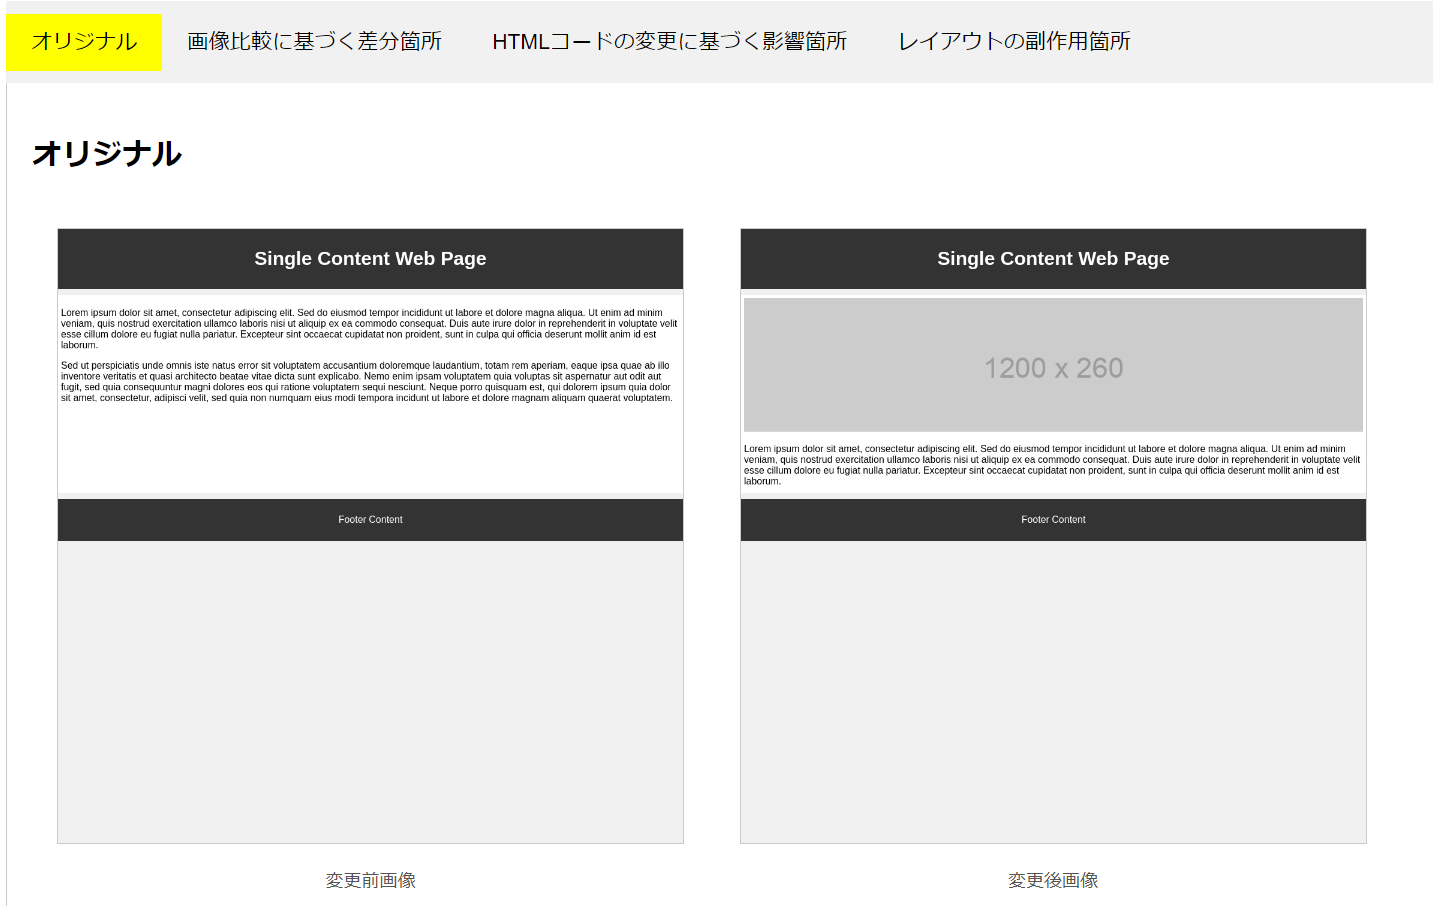
\includegraphics[width=1.0\columnwidth]{image/3_Appearance.png}
        \caption{\toolName の外観}
        \label{fig: Appearance}
    \end{center}
\end{figure}
% \toolName は、以下に示す4つのタブからなるタブメニューと各タブに対応した内容を表示するタブコンテンツからなる。
% なお、以下の数字は、図\ref{fig: Appearance}の数字と対応している。
% \begin{itemize}
%     \item タブメニュー
%     \item タブコンテンツ
% \end{itemize}
% \par
% また、タブメニューを構成する4つのタブは以下の通りである。
% \begin{itemize}
%     \item [①]オリジナル画像表示タブ
%     \item [②]画像比較に基づく差分箇所表示タブ
%     \item [③]HTMLコードの変更に基づく影響箇所表示タブ
%     \item [④]レイアウトの副作用箇所表示タブ
% \end{itemize}
% \par
% 以降、各タブの外観と機能について説明する。
% Webアプリケーションとして試作した\toolName は、以下に示す4つのタブからなるタブメニューと各タブに対応した内容を表示するタブコンテンツからなる。
% なお、以下の数字は、図\ref{fig: Appearance}の数字と対応している。
\toolName は、以下に示す4つのタブからなるタブメニューと各タブに対応した内容を表示するタブコンテンツからなる。
なお、以下の数字は、図\ref{fig: Appearance}の数字と対応している。
\begin{itemize}
    \item[①] タブメニュー
          \begin{itemize}
              \item オリジナル表示タブ
              \item 画像比較に基づく差分箇所表示タブ
              \item HTMLコードの変更に基づく影響箇所表示タブ
              \item レイアウトの副作用箇所表示タブ
          \end{itemize}
    \item[②] タブコンテンツ
\end{itemize}
\par
以降、各タブの外観と機能について説明する。



\section{オリジナル表示タブ}\label{subsec:original_tab}
オリジナル表示タブを押すと、Webページの変更前画像とWebページの変更後画像を表示する。
オリジナル表示タブを押した際の\toolName の画面例を、図\ref{fig: Appearance_original_tab}に示す。
なお、\toolName に一番最初にアクセスした時やリロードした時に、デフォルトでオリジナル表示タブを選択した状態になっている。
このタブでは、Webページの変更前後の画像を目視で確認できる。
\begin{figure}[tp]
    \begin{center}
        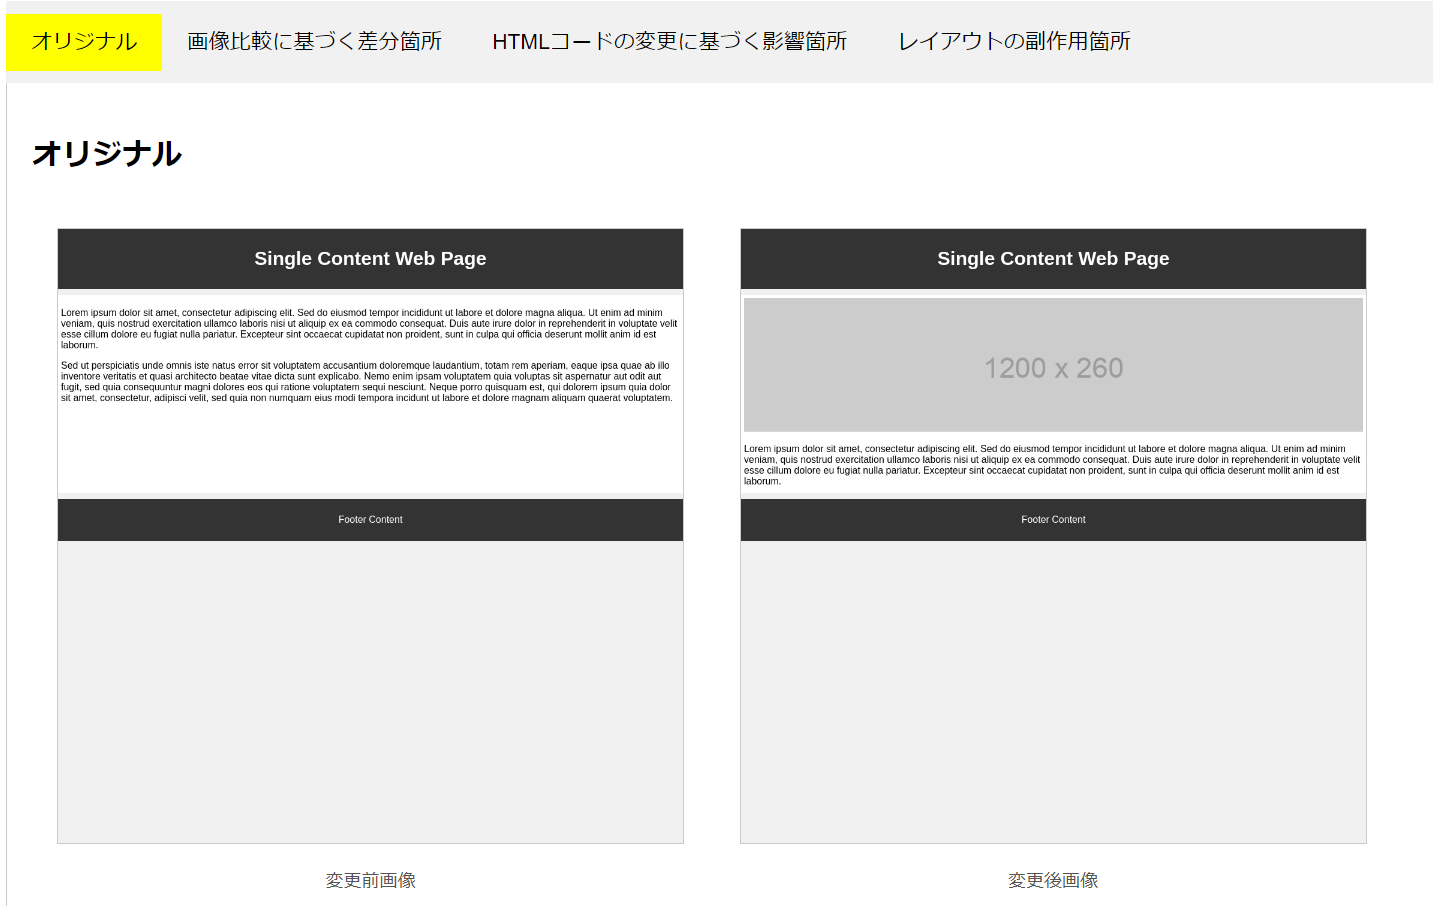
\includegraphics[width=1.0\columnwidth]{image/3_original_tab.png}
        \caption{オリジナル表示タブを押した際の\toolName の画面例}
        \label{fig: Appearance_original_tab}
    \end{center}
\end{figure}



\section{画像比較に基づく差分箇所表示タブ}\label{subsec:images_tab}
画像比較に基づく差分箇所表示タブを押すと、画像比較に基づく差分箇所を色付きの枠で囲んで強調表示した、Webページの変更前画像とWebページの変更後画像を表示する。
画像比較に基づく差分箇所表示タブを押した際の\toolName の画面例を、図\ref{fig: Appearance_images_tab}に示す。
ここでの差分箇所とは、変更前後のWebページを比較して、変更前のWebページで削除された箇所と変更後のWebページで追加された箇所を差分箇所と定義する。
削除された箇所は変更前画像上に赤枠で囲んで強調表示し、追加された箇所は変更後画像上に緑枠で囲んで強調表示する。
このタブでは、変更前後のWebページで画素単位での見た目の差分があった箇所を目視で確認できる。
\begin{figure}[tp]
    \begin{center}
        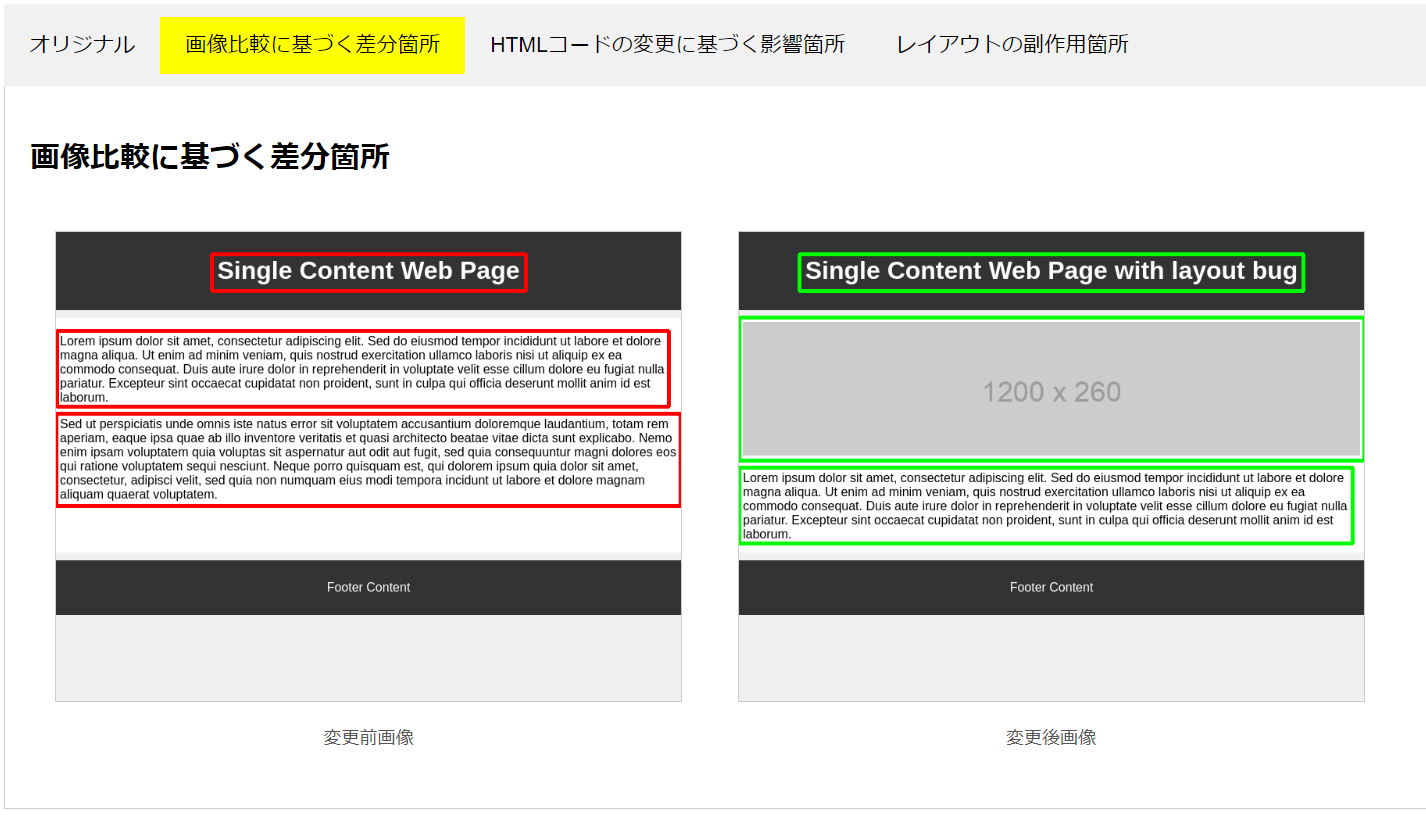
\includegraphics[width=1.0\columnwidth]{image/3_images_tab.png}
        \caption{画像比較に基づく差分箇所表示タブを押した際の\toolName の画面例}
        \label{fig: Appearance_images_tab}
    \end{center}
\end{figure}



\section{HTMLコードの変更に基づく影響箇所表示タブ}\label{subsec:html_tab}
HTMLの変更に基づく影響箇所表示タブを押すと、HTMLの変更に基づく影響箇所を色付きの枠で囲んで強調表示した、Webページの変更前画像とWebページの変更後画像を表示する。
HTMLの変更に基づく影響箇所表示タブを押した際の画面例を、図\ref{fig: Appearance_html_tab}に示す。
ここでの影響箇所とは、変更前後のWebページのHTMLコードを比較して、HTMLコードにおけるbody要素内の変更とstyle要素内の変更のどちらか、または両方の影響を受けた画面要素箇所と定義する。
変更前のWebページのHTMLでの影響箇所は変更前画像上に赤枠で囲んで強調表示し、変更後のWebページのHTMLでの影響箇所は変更後画像上に緑枠で囲んで強調表示する。
また、変更前画像上の赤枠内の左上に「影響箇所です」という赤色のテキストと、変更後画像上の緑枠内の左上に「影響箇所です」という緑色のテキストを表示することで、
より視覚的に影響箇所の位置を強調する。
このタブでは、図\ref{fig: Appearance_images_tab}における差分箇所から、開発者が意図して変更した、または意図せず変更してしまったHTMLコードによる影響箇所を目視で確認できる。
% このタブでは、変更前後のWebページで開発者が意図した、または意図しないHTMLコードの変更による影響箇所を目視で確認できる。
\begin{figure}[tp]
    \begin{center}
        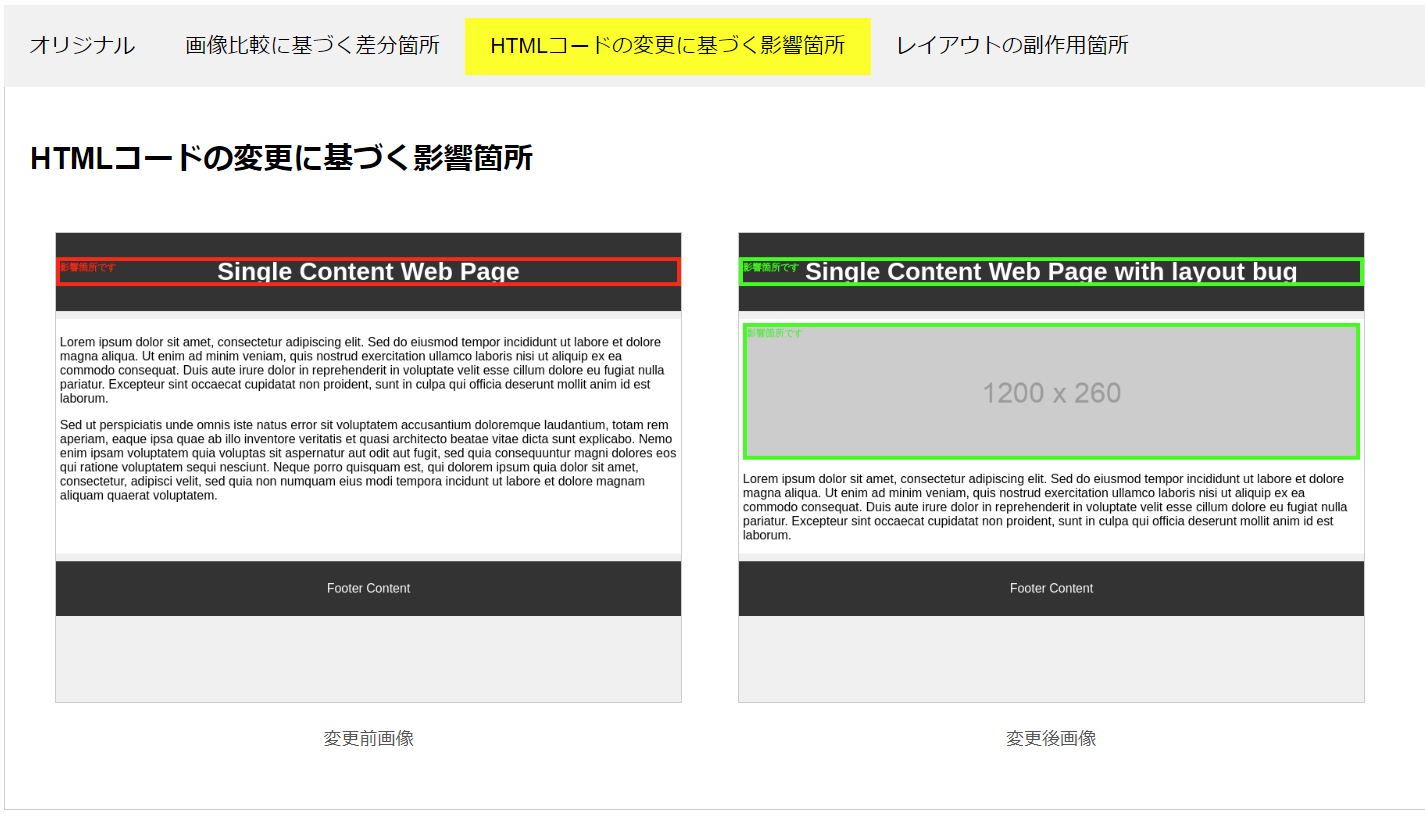
\includegraphics[width=1.0\columnwidth]{image/3_html_tab.png}
        \caption{HTMLコードの変更に基づく影響箇所表示タブを押した際の\toolName の画面例}
        \label{fig: Appearance_html_tab}
    \end{center}
\end{figure}



\section{レイアウトの副作用箇所表示タブ}\label{subsec:subeffect_tab}
レイアウトの副作用箇所表示タブを押すと、差分箇所と影響箇所に基づいて出力したレイアウトの副作用箇所を色付きの枠で強調表示した、Webページの変更前画像とWebページの変更後画像を表示する。
レイアウトの副作用箇所表示タブを押した際の画面例を、図\ref{fig: Appearance_subEffect_tab}に示す。
ここでのレイアウトの副作用箇所とは、変更前後のWebページでHTMLコードの変更による影響を受けた画面要素によって、HTMLコードを変更していない画面要素に見た目の変更があった箇所と定義する。
変更前のWebページでのレイアウトの副作用箇所は変更前画像上に赤枠で囲んで強調表示し、変更後のwebページでのレイアウトの副作用箇所は変更後画像上に緑枠で囲んで強調表示する。
このタブでは、図\ref{fig: Appearance_images_tab}における差分箇所から、レイアウトの不具合を含む可能性のある箇所を目視で確認できる。
\begin{figure}[tp]
    \begin{center}
        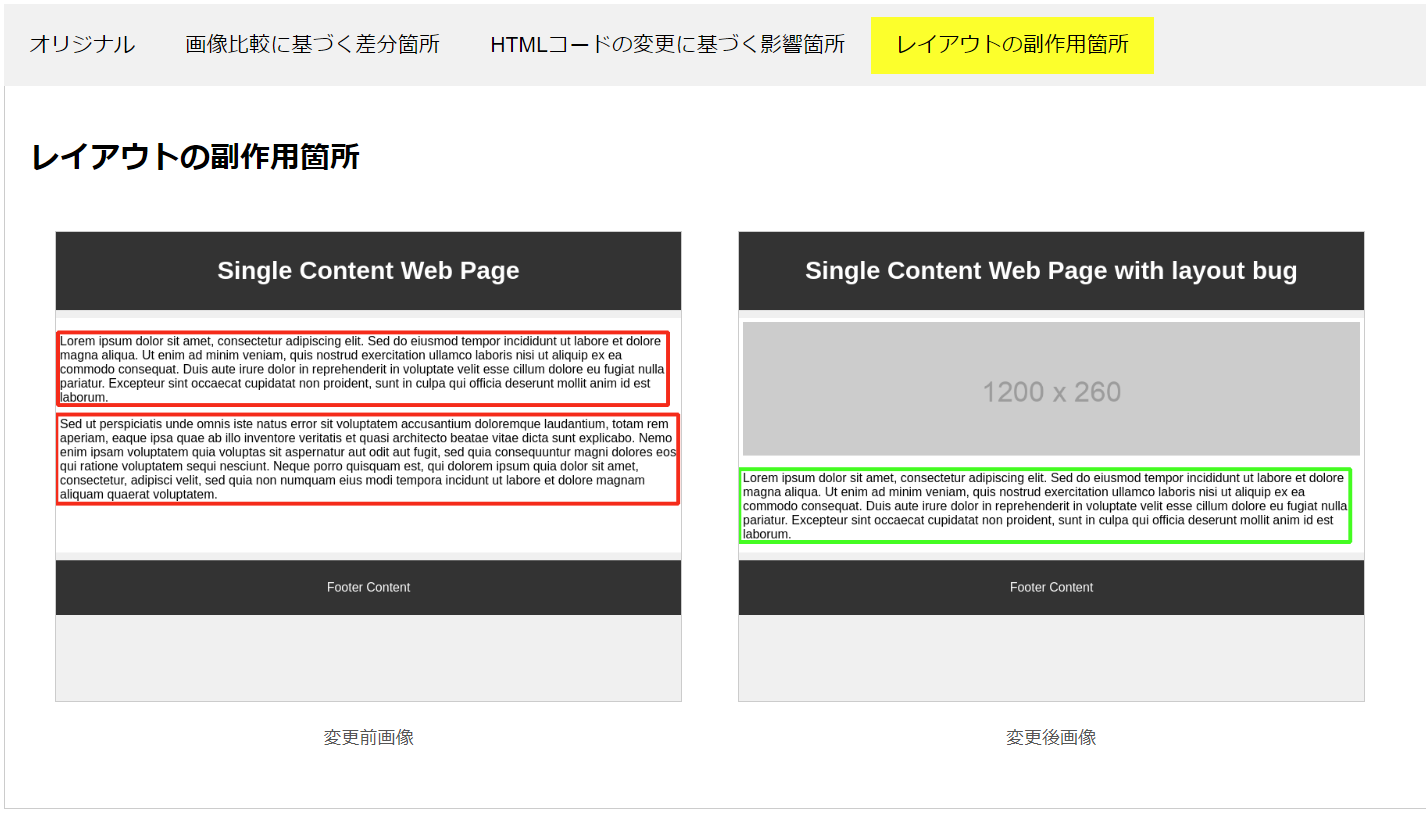
\includegraphics[width=1.0\columnwidth]{image/3_subEffect_tab.png}
        \caption{レイアウトの副作用箇所表示タブを押した際の\toolName の画面例}
        \label{fig: Appearance_subEffect_tab}
    \end{center}
\end{figure}

